\section{Ziel}
In diesem Versuch soll eine Kuper-Röntgenröhre auf ihr Emissionsspektrum untersucht und die Bragg-Bedingung überprüft werden.
Außerdem sollen diverse Absorptionsspektren gemessen und ihre Abschirmkonstanten bestimmmt werden.


\section[Theorie]{Theorie\footnote[1]{Unter Verwendung von \cite[]{man:v602}.}}

\subsection{Erzeugung von Röntgenstrahlung}
Röntgenstrahlung wird erzeugt, indem in einer evakuierten Röhre Elektronen durch den glühelektrischen Effekt aus einer Kathode gelöst werden.
Diese Elektronen werden durch eine angelegte Spannung zu einer Anode hin beschleunigt.
Beim Auftreffen auf die Anode entsteht Röntgenstrahlung, wobei das kontinuierliche Bremsspekttrum und die diskrete charakteristische Röntgenstrahlung des Anodenmaterials unterschieden werden.

\noindent
Bei der Bremsstrahlung werden die Elektronen im Coulombfeld des positives Atomkerns abgebremst.
Durch die Abremsung wird ein Photon emittiert, dessen Energie genau der verloren kinetischen Energie des jeweiligen Elektrons entspricht.
Da nicht alle Elektronen die gleiche Energie abgeben, entsteht ein kontinuierliches Energiespektrum, das eine obere Grenze an der Stelle hat,
bei der die gesamte kinetische Energie übertragen wird.
Für die minimale Wellenlänge folgt demnach bei vollständiger Abbremsung des Elektrons
\begin{align}
    \lambda_\text{min} = \frac{h \cdot c}{e_0 U},
    \label{eq:wellenlaenge}
\end{align}
wobei $U$ die angelegt Spannung ist.
Die Intensitätsverteilung des Bresmspektrums ist in Abbildung \ref{fig:bremsspektrum} zu sehen.

\noindent
Beim charakteristischen Spektrum werden die Anodenatome so ionisiert, dass das beschleunigte Elektron 
ein inneres Schalenelektron heraus löst. 
Wenn das Atom anschließend in seinen Grundzustand zurück wechselt, wird ein Photon mit der Energie 
\begin{align}
    \Delta E = h \cdot \nu = E_\text{m} - E_\text{n}
    \label{eq:energiedifferenz}
\end{align}
emittiert.
Diese Energie entspricht genau der Energiedifferenz der der äußeren Schale m, von der ein Elektron nachrückt, und der inneren Schale n,
aus der das Elektron geschlagen wurde. 

\begin{figure}[H]
    \centering
    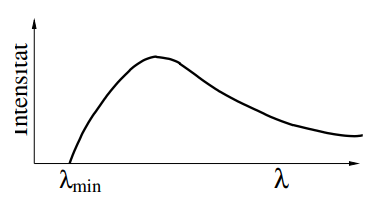
\includegraphics[height = 3.5cm]{Abbildungen/bremsspektrum.png}
    \caption{Intensitätsverteilung in Abhängigkeit der Wellenlänge beim charakteristischen Spektrum \cite[]{man:v602}.}
    \label{fig:bremsspektrum}
\end{figure}